
% Default to the notebook output style

    


% Inherit from the specified cell style.




    
% \documentclass{article}

    
    
%     \usepackage{graphicx} % Used to insert images
%     \usepackage{adjustbox} % Used to constrain images to a maximum size 
%     \usepackage{color} % Allow colors to be defined
%     \usepackage{enumerate} % Needed for markdown enumerations to work
%     \usepackage{geometry} % Used to adjust the document margins
%     \usepackage{amsmath} % Equations
%     \usepackage{amssymb} % Equations
%     \usepackage[mathletters]{ucs} % Extended unicode (utf-8) support
%     \usepackage[utf8x]{inputenc} % Allow utf-8 characters in the tex document
%     \usepackage{fancyvrb} % verbatim replacement that allows latex
%     \usepackage{grffile} % extends the file name processing of package graphics 
%                          % to support a larger range 
%     % The hyperref package gives us a pdf with properly built
%     % internal navigation ('pdf bookmarks' for the table of contents,
%     % internal cross-reference links, web links for URLs, etc.)
%     \usepackage{hyperref}
%     \usepackage{longtable} % longtable support required by pandoc >1.10
    

    
    
    \definecolor{orange}{cmyk}{0,0.4,0.8,0.2}
    \definecolor{darkorange}{rgb}{.71,0.21,0.01}
    \definecolor{darkgreen}{rgb}{.12,.54,.11}
    \definecolor{myteal}{rgb}{.26, .44, .56}
    \definecolor{gray}{gray}{0.45}
    \definecolor{lightgray}{gray}{.95}
    \definecolor{mediumgray}{gray}{.8}
    \definecolor{inputbackground}{rgb}{.95, .95, .85}
    \definecolor{outputbackground}{rgb}{.95, .95, .95}
    \definecolor{traceback}{rgb}{1, .95, .95}
    % ansi colors
    \definecolor{red}{rgb}{.6,0,0}
    \definecolor{green}{rgb}{0,.65,0}
    \definecolor{brown}{rgb}{0.6,0.6,0}
    \definecolor{blue}{rgb}{0,.145,.698}
    \definecolor{purple}{rgb}{.698,.145,.698}
    \definecolor{cyan}{rgb}{0,.698,.698}
    \definecolor{lightgray}{gray}{0.5}
    
    % bright ansi colors
    \definecolor{darkgray}{gray}{0.25}
    \definecolor{lightred}{rgb}{1.0,0.39,0.28}
    \definecolor{lightgreen}{rgb}{0.48,0.99,0.0}
    \definecolor{lightblue}{rgb}{0.53,0.81,0.92}
    \definecolor{lightpurple}{rgb}{0.87,0.63,0.87}
    \definecolor{lightcyan}{rgb}{0.5,1.0,0.83}
    
    % commands and environments needed by pandoc snippets
    % extracted from the output of `pandoc -s`
    \DefineVerbatimEnvironment{Highlighting}{Verbatim}{commandchars=\\\{\}}
    % Add ',fontsize=\small' for more characters per line
    \newenvironment{Shaded}{}{}
    \newcommand{\KeywordTok}[1]{\textcolor[rgb]{0.00,0.44,0.13}{\textbf{{#1}}}}
    \newcommand{\DataTypeTok}[1]{\textcolor[rgb]{0.56,0.13,0.00}{{#1}}}
    \newcommand{\DecValTok}[1]{\textcolor[rgb]{0.25,0.63,0.44}{{#1}}}
    \newcommand{\BaseNTok}[1]{\textcolor[rgb]{0.25,0.63,0.44}{{#1}}}
    \newcommand{\FloatTok}[1]{\textcolor[rgb]{0.25,0.63,0.44}{{#1}}}
    \newcommand{\CharTok}[1]{\textcolor[rgb]{0.25,0.44,0.63}{{#1}}}
    \newcommand{\StringTok}[1]{\textcolor[rgb]{0.25,0.44,0.63}{{#1}}}
    \newcommand{\CommentTok}[1]{\textcolor[rgb]{0.38,0.63,0.69}{\textit{{#1}}}}
    \newcommand{\OtherTok}[1]{\textcolor[rgb]{0.00,0.44,0.13}{{#1}}}
    \newcommand{\AlertTok}[1]{\textcolor[rgb]{1.00,0.00,0.00}{\textbf{{#1}}}}
    \newcommand{\FunctionTok}[1]{\textcolor[rgb]{0.02,0.16,0.49}{{#1}}}
    \newcommand{\RegionMarkerTok}[1]{{#1}}
    \newcommand{\ErrorTok}[1]{\textcolor[rgb]{1.00,0.00,0.00}{\textbf{{#1}}}}
    \newcommand{\NormalTok}[1]{{#1}}
    
    % Define a nice break command that doesn't care if a line doesn't already
    % exist.
    \def\br{\hspace*{\fill} \\* }
    % Math Jax compatability definitions
    \def\gt{>}
    \def\lt{<}
    % Document parameters
    \title{BAK4\_final}
    
    
    

    % Pygments definitions
    
\makeatletter
\def\PY@reset{\let\PY@it=\relax \let\PY@bf=\relax%
    \let\PY@ul=\relax \let\PY@tc=\relax%
    \let\PY@bc=\relax \let\PY@ff=\relax}
\def\PY@tok#1{\csname PY@tok@#1\endcsname}
\def\PY@toks#1+{\ifx\relax#1\empty\else%
    \PY@tok{#1}\expandafter\PY@toks\fi}
\def\PY@do#1{\PY@bc{\PY@tc{\PY@ul{%
    \PY@it{\PY@bf{\PY@ff{#1}}}}}}}
\def\PY#1#2{\PY@reset\PY@toks#1+\relax+\PY@do{#2}}

\expandafter\def\csname PY@tok@gd\endcsname{\def\PY@tc##1{\textcolor[rgb]{0.63,0.00,0.00}{##1}}}
\expandafter\def\csname PY@tok@gu\endcsname{\let\PY@bf=\textbf\def\PY@tc##1{\textcolor[rgb]{0.50,0.00,0.50}{##1}}}
\expandafter\def\csname PY@tok@gt\endcsname{\def\PY@tc##1{\textcolor[rgb]{0.00,0.27,0.87}{##1}}}
\expandafter\def\csname PY@tok@gs\endcsname{\let\PY@bf=\textbf}
\expandafter\def\csname PY@tok@gr\endcsname{\def\PY@tc##1{\textcolor[rgb]{1.00,0.00,0.00}{##1}}}
\expandafter\def\csname PY@tok@cm\endcsname{\let\PY@it=\textit\def\PY@tc##1{\textcolor[rgb]{0.25,0.50,0.50}{##1}}}
\expandafter\def\csname PY@tok@vg\endcsname{\def\PY@tc##1{\textcolor[rgb]{0.10,0.09,0.49}{##1}}}
\expandafter\def\csname PY@tok@m\endcsname{\def\PY@tc##1{\textcolor[rgb]{0.40,0.40,0.40}{##1}}}
\expandafter\def\csname PY@tok@mh\endcsname{\def\PY@tc##1{\textcolor[rgb]{0.40,0.40,0.40}{##1}}}
\expandafter\def\csname PY@tok@go\endcsname{\def\PY@tc##1{\textcolor[rgb]{0.53,0.53,0.53}{##1}}}
\expandafter\def\csname PY@tok@ge\endcsname{\let\PY@it=\textit}
\expandafter\def\csname PY@tok@vc\endcsname{\def\PY@tc##1{\textcolor[rgb]{0.10,0.09,0.49}{##1}}}
\expandafter\def\csname PY@tok@il\endcsname{\def\PY@tc##1{\textcolor[rgb]{0.40,0.40,0.40}{##1}}}
\expandafter\def\csname PY@tok@cs\endcsname{\let\PY@it=\textit\def\PY@tc##1{\textcolor[rgb]{0.25,0.50,0.50}{##1}}}
\expandafter\def\csname PY@tok@cp\endcsname{\def\PY@tc##1{\textcolor[rgb]{0.74,0.48,0.00}{##1}}}
\expandafter\def\csname PY@tok@gi\endcsname{\def\PY@tc##1{\textcolor[rgb]{0.00,0.63,0.00}{##1}}}
\expandafter\def\csname PY@tok@gh\endcsname{\let\PY@bf=\textbf\def\PY@tc##1{\textcolor[rgb]{0.00,0.00,0.50}{##1}}}
\expandafter\def\csname PY@tok@ni\endcsname{\let\PY@bf=\textbf\def\PY@tc##1{\textcolor[rgb]{0.60,0.60,0.60}{##1}}}
\expandafter\def\csname PY@tok@nl\endcsname{\def\PY@tc##1{\textcolor[rgb]{0.63,0.63,0.00}{##1}}}
\expandafter\def\csname PY@tok@nn\endcsname{\let\PY@bf=\textbf\def\PY@tc##1{\textcolor[rgb]{0.00,0.00,1.00}{##1}}}
\expandafter\def\csname PY@tok@no\endcsname{\def\PY@tc##1{\textcolor[rgb]{0.53,0.00,0.00}{##1}}}
\expandafter\def\csname PY@tok@na\endcsname{\def\PY@tc##1{\textcolor[rgb]{0.49,0.56,0.16}{##1}}}
\expandafter\def\csname PY@tok@nb\endcsname{\def\PY@tc##1{\textcolor[rgb]{0.00,0.50,0.00}{##1}}}
\expandafter\def\csname PY@tok@nc\endcsname{\let\PY@bf=\textbf\def\PY@tc##1{\textcolor[rgb]{0.00,0.00,1.00}{##1}}}
\expandafter\def\csname PY@tok@nd\endcsname{\def\PY@tc##1{\textcolor[rgb]{0.67,0.13,1.00}{##1}}}
\expandafter\def\csname PY@tok@ne\endcsname{\let\PY@bf=\textbf\def\PY@tc##1{\textcolor[rgb]{0.82,0.25,0.23}{##1}}}
\expandafter\def\csname PY@tok@nf\endcsname{\def\PY@tc##1{\textcolor[rgb]{0.00,0.00,1.00}{##1}}}
\expandafter\def\csname PY@tok@si\endcsname{\let\PY@bf=\textbf\def\PY@tc##1{\textcolor[rgb]{0.73,0.40,0.53}{##1}}}
\expandafter\def\csname PY@tok@s2\endcsname{\def\PY@tc##1{\textcolor[rgb]{0.73,0.13,0.13}{##1}}}
\expandafter\def\csname PY@tok@vi\endcsname{\def\PY@tc##1{\textcolor[rgb]{0.10,0.09,0.49}{##1}}}
\expandafter\def\csname PY@tok@nt\endcsname{\let\PY@bf=\textbf\def\PY@tc##1{\textcolor[rgb]{0.00,0.50,0.00}{##1}}}
\expandafter\def\csname PY@tok@nv\endcsname{\def\PY@tc##1{\textcolor[rgb]{0.10,0.09,0.49}{##1}}}
\expandafter\def\csname PY@tok@s1\endcsname{\def\PY@tc##1{\textcolor[rgb]{0.73,0.13,0.13}{##1}}}
\expandafter\def\csname PY@tok@sh\endcsname{\def\PY@tc##1{\textcolor[rgb]{0.73,0.13,0.13}{##1}}}
\expandafter\def\csname PY@tok@sc\endcsname{\def\PY@tc##1{\textcolor[rgb]{0.73,0.13,0.13}{##1}}}
\expandafter\def\csname PY@tok@sx\endcsname{\def\PY@tc##1{\textcolor[rgb]{0.00,0.50,0.00}{##1}}}
\expandafter\def\csname PY@tok@bp\endcsname{\def\PY@tc##1{\textcolor[rgb]{0.00,0.50,0.00}{##1}}}
\expandafter\def\csname PY@tok@c1\endcsname{\let\PY@it=\textit\def\PY@tc##1{\textcolor[rgb]{0.25,0.50,0.50}{##1}}}
\expandafter\def\csname PY@tok@kc\endcsname{\let\PY@bf=\textbf\def\PY@tc##1{\textcolor[rgb]{0.00,0.50,0.00}{##1}}}
\expandafter\def\csname PY@tok@c\endcsname{\let\PY@it=\textit\def\PY@tc##1{\textcolor[rgb]{0.25,0.50,0.50}{##1}}}
\expandafter\def\csname PY@tok@mf\endcsname{\def\PY@tc##1{\textcolor[rgb]{0.40,0.40,0.40}{##1}}}
\expandafter\def\csname PY@tok@err\endcsname{\def\PY@bc##1{\setlength{\fboxsep}{0pt}\fcolorbox[rgb]{1.00,0.00,0.00}{1,1,1}{\strut ##1}}}
\expandafter\def\csname PY@tok@kd\endcsname{\let\PY@bf=\textbf\def\PY@tc##1{\textcolor[rgb]{0.00,0.50,0.00}{##1}}}
\expandafter\def\csname PY@tok@ss\endcsname{\def\PY@tc##1{\textcolor[rgb]{0.10,0.09,0.49}{##1}}}
\expandafter\def\csname PY@tok@sr\endcsname{\def\PY@tc##1{\textcolor[rgb]{0.73,0.40,0.53}{##1}}}
\expandafter\def\csname PY@tok@mo\endcsname{\def\PY@tc##1{\textcolor[rgb]{0.40,0.40,0.40}{##1}}}
\expandafter\def\csname PY@tok@kn\endcsname{\let\PY@bf=\textbf\def\PY@tc##1{\textcolor[rgb]{0.00,0.50,0.00}{##1}}}
\expandafter\def\csname PY@tok@mi\endcsname{\def\PY@tc##1{\textcolor[rgb]{0.40,0.40,0.40}{##1}}}
\expandafter\def\csname PY@tok@gp\endcsname{\let\PY@bf=\textbf\def\PY@tc##1{\textcolor[rgb]{0.00,0.00,0.50}{##1}}}
\expandafter\def\csname PY@tok@o\endcsname{\def\PY@tc##1{\textcolor[rgb]{0.40,0.40,0.40}{##1}}}
\expandafter\def\csname PY@tok@kr\endcsname{\let\PY@bf=\textbf\def\PY@tc##1{\textcolor[rgb]{0.00,0.50,0.00}{##1}}}
\expandafter\def\csname PY@tok@s\endcsname{\def\PY@tc##1{\textcolor[rgb]{0.73,0.13,0.13}{##1}}}
\expandafter\def\csname PY@tok@kp\endcsname{\def\PY@tc##1{\textcolor[rgb]{0.00,0.50,0.00}{##1}}}
\expandafter\def\csname PY@tok@w\endcsname{\def\PY@tc##1{\textcolor[rgb]{0.73,0.73,0.73}{##1}}}
\expandafter\def\csname PY@tok@kt\endcsname{\def\PY@tc##1{\textcolor[rgb]{0.69,0.00,0.25}{##1}}}
\expandafter\def\csname PY@tok@ow\endcsname{\let\PY@bf=\textbf\def\PY@tc##1{\textcolor[rgb]{0.67,0.13,1.00}{##1}}}
\expandafter\def\csname PY@tok@sb\endcsname{\def\PY@tc##1{\textcolor[rgb]{0.73,0.13,0.13}{##1}}}
\expandafter\def\csname PY@tok@k\endcsname{\let\PY@bf=\textbf\def\PY@tc##1{\textcolor[rgb]{0.00,0.50,0.00}{##1}}}
\expandafter\def\csname PY@tok@se\endcsname{\let\PY@bf=\textbf\def\PY@tc##1{\textcolor[rgb]{0.73,0.40,0.13}{##1}}}
\expandafter\def\csname PY@tok@sd\endcsname{\let\PY@it=\textit\def\PY@tc##1{\textcolor[rgb]{0.73,0.13,0.13}{##1}}}

\def\PYZbs{\char`\\}
\def\PYZus{\char`\_}
\def\PYZob{\char`\{}
\def\PYZcb{\char`\}}
\def\PYZca{\char`\^}
\def\PYZam{\char`\&}
\def\PYZlt{\char`\<}
\def\PYZgt{\char`\>}
\def\PYZsh{\char`\#}
\def\PYZpc{\char`\%}
\def\PYZdl{\char`\$}
\def\PYZhy{\char`\-}
\def\PYZsq{\char`\'}
\def\PYZdq{\char`\"}
\def\PYZti{\char`\~}
% for compatibility with earlier versions
\def\PYZat{@}
\def\PYZlb{[}
\def\PYZrb{]}
\makeatother


    % Exact colors from NB
    \definecolor{incolor}{rgb}{0.0, 0.0, 0.5}
    \definecolor{outcolor}{rgb}{0.545, 0.0, 0.0}



    
    % Prevent overflowing lines due to hard-to-break entities
    \sloppy 
    % Setup hyperref package
    \hypersetup{
      breaklinks=true,  % so long urls are correctly broken across lines
      colorlinks=true,
      urlcolor=blue,
      linkcolor=darkorange,
      citecolor=darkgreen,
      }
    % Slightly bigger margins than the latex defaults
    
    % \geometry{verbose,tmargin=1in,bmargin=1in,lmargin=1in,rmargin=1in}
    
    

    % \begin{document}
    
    
    % \maketitle
    
    

    
\section{Documentation of Python Peak Detection Code }
\label{sec:python}


                
    This is a walkthrough of the proposed peak detection python code. This code is the basis for the script in Appendix ~\ref{pythonMaxCode}, which actually can be run inside Max/MSP to compute the resonance
frequencies.


 \subsection{Setup and Data import}
\label{subsec:setup}
Some external modules are loaded first.

    \begin{Verbatim}[commandchars=\\\{\}]
{\color{incolor}In [{\color{incolor}23}]:} \PY{o}{\PYZpc{}}\PY{k}{matplotlib} \PY{n}{inline}
         \PY{k+kn}{import} \PY{n+nn}{matplotlib.pyplot} \PY{k+kn}{as} \PY{n+nn}{plt}
         \PY{k+kn}{import} \PY{n+nn}{numpy} \PY{k+kn}{as} \PY{n+nn}{np}
\end{Verbatim}

%     set working directory:

%     \begin{Verbatim}[commandchars=\\\{\}]
% {\color{incolor}In [{\color{incolor}24}]:} \PY{n}{cd} \PY{o}{/}\PY{n}{Users}\PY{o}{/}\PY{n}{macuserin}\PY{o}{/}\PY{n}{Documents}\PY{o}{/}\PY{n}{Max}\PY{o}{/}\PY{n}{Projects}\PY{o}{/}\PY{n}{BAC3}\PY{o}{/}\PY{n}{data}
% \end{Verbatim}

%     \begin{Verbatim}[commandchars=\\\{\}]
% /Users/macuserin/Documents/Max/Projects/BAC3/data
%     \end{Verbatim}

    Audio and spectral processing is done inside Max/MSP. Since it's easily
possible to save the magnitude data as a JSON file for the purpose of
demonstrating the proposed algorithm, a JSON-parsing helper function is
written here:

    \begin{Verbatim}[commandchars=\\\{\}]
{\color{incolor}In [{\color{incolor}25}]:} \PY{k}{def} \PY{n+nf}{parseFrame}\PY{p}{(}\PY{n}{jsonFile}\PY{p}{)}\PY{p}{:}
             \PY{k+kn}{import} \PY{n+nn}{json}
             \PY{n}{json\PYZus{}data}\PY{o}{=}\PY{n+nb}{open}\PY{p}{(}\PY{n}{jsonFile}\PY{p}{)}
             \PY{n}{data} \PY{o}{=} \PY{n}{json}\PY{o}{.}\PY{n}{load}\PY{p}{(}\PY{n}{json\PYZus{}data}\PY{p}{)}
             \PY{n}{json\PYZus{}data}\PY{o}{.}\PY{n}{close}\PY{p}{(}\PY{p}{)}
             \PY{n}{array1} \PY{o}{=} \PY{p}{[}\PY{p}{]}
             \PY{k}{for} \PY{n}{i} \PY{o+ow}{in} \PY{n+nb}{range} \PY{p}{(}\PY{n+nb}{len}\PY{p}{(}\PY{n}{data}\PY{p}{)}\PY{p}{)}\PY{p}{:}
                 \PY{n}{array1}\PY{o}{.}\PY{n}{append}\PY{p}{(}\PY{n}{data}\PY{p}{[}\PY{n+nb}{str}\PY{p}{(}\PY{n}{i}\PY{p}{)}\PY{p}{]}\PY{p}{[}\PY{l+m+mi}{0}\PY{p}{]}\PY{p}{)}
             \PY{k}{return} \PY{n}{array1}
\end{Verbatim}

    Here, the accumulation of the autocorrelation's spectrum is loaded and
some constants are set:

    \begin{Verbatim}[commandchars=\\\{\}]
{\color{incolor}In [{\color{incolor}26}]:} \PY{n}{spectrum} \PY{o}{=} \PY{n}{parseFrame}\PY{p}{(}\PY{l+s}{\PYZdq{}}\PY{l+s}{Kuebel\PYZus{}Acc\PYZus{}autoCorrel.json}\PY{l+s}{\PYZdq{}}\PY{p}{)}
         \PY{n}{sr} \PY{o}{=} \PY{l+m+mf}{44100.}
         \PY{n}{frameSize} \PY{o}{=} \PY{n+nb}{len}\PY{p}{(}\PY{n}{spectrum}\PY{p}{)}
\end{Verbatim}

    Helper function to convert a bin number to a frequency in Hz:

    \begin{Verbatim}[commandchars=\\\{\}]
{\color{incolor}In [{\color{incolor}27}]:} \PY{k}{def} \PY{n+nf}{binToFreq}\PY{p}{(}\PY{n}{bins}\PY{p}{,} \PY{n}{sr}\PY{p}{,} \PY{n}{frameSize}\PY{p}{)}\PY{p}{:}
             \PY{n}{freqs} \PY{o}{=} \PY{p}{[}\PY{p}{]}
             \PY{k}{for} \PY{n}{i} \PY{o+ow}{in} \PY{n+nb}{range}\PY{p}{(}\PY{n+nb}{len}\PY{p}{(}\PY{n}{bins}\PY{p}{)}\PY{p}{)}\PY{p}{:}
                 \PY{n}{f} \PY{o}{=} \PY{p}{(}\PY{n}{bins}\PY{p}{[}\PY{n}{i}\PY{p}{]}\PY{o}{/}\PY{n+nb}{float}\PY{p}{(}\PY{n}{frameSize}\PY{p}{)}\PY{p}{)}\PY{o}{*}\PY{n}{sr}\PY{o}{/}\PY{l+m+mi}{2}
                 \PY{n}{freqs}\PY{o}{.}\PY{n}{append}\PY{p}{(}\PY{n}{f}\PY{p}{)}
             \PY{k}{return} \PY{n}{freqs}
\end{Verbatim}

    Below, just the raw loaded data is plotted:

    \begin{Verbatim}[commandchars=\\\{\}]
{\color{incolor}In [{\color{incolor}28}]:} \PY{n}{fig} \PY{o}{=} \PY{n}{plt}\PY{o}{.}\PY{n}{figure}\PY{p}{(}\PY{n}{figsize}\PY{o}{=}\PY{p}{(}\PY{l+m+mi}{10}\PY{p}{,}\PY{l+m+mi}{5}\PY{p}{)}\PY{p}{)}
         \PY{n}{ax} \PY{o}{=} \PY{n}{fig}\PY{o}{.}\PY{n}{add\PYZus{}subplot}\PY{p}{(}\PY{l+m+mi}{111}\PY{p}{)}
         \PY{n}{frame} \PY{o}{=} \PY{n}{spectrum}
         \PY{n}{n} \PY{o}{=} \PY{n}{np}\PY{o}{.}\PY{n}{linspace}\PY{p}{(}\PY{l+m+mi}{0}\PY{p}{,} \PY{n}{sr}\PY{o}{/}\PY{l+m+mi}{2}\PY{p}{,} \PY{n}{frameSize}\PY{p}{)}
         \PY{n}{plt}\PY{o}{.}\PY{n}{plot}\PY{p}{(}\PY{n}{n}\PY{p}{,} \PY{n}{frame}\PY{p}{)}
         \PY{n}{plt}\PY{o}{.}\PY{n}{title}\PY{p}{(}\PY{l+s}{\PYZsq{}}\PY{l+s}{Accumulation of the Spectrum of the Autocorrelation}\PY{l+s}{\PYZsq{}}\PY{p}{)}\PY{p}{;}
         \PY{n}{plt}\PY{o}{.}\PY{n}{axis}\PY{p}{(}\PY{p}{[}\PY{l+m+mi}{0}\PY{p}{,} \PY{n}{sr}\PY{o}{/}\PY{l+m+mi}{2}\PY{p}{,} \PY{l+m+mi}{0}\PY{p}{,} \PY{l+m+mf}{1.2}\PY{p}{]}\PY{p}{)}
         \PY{n}{ax}\PY{o}{.}\PY{n}{set\PYZus{}xlabel}\PY{p}{(}\PY{l+s}{\PYZsq{}}\PY{l+s}{frequency}\PY{l+s}{\PYZsq{}}\PY{p}{)}
         \PY{n}{ax}\PY{o}{.}\PY{n}{set\PYZus{}ylabel}\PY{p}{(}\PY{l+s}{\PYZsq{}}\PY{l+s}{Linear Ampitude}\PY{l+s}{\PYZsq{}}\PY{p}{)}
\end{Verbatim}

%             \begin{Verbatim}[commandchars=\\\{\}]
% {\color{outcolor}Out[{\color{outcolor}28}]:} <matplotlib.text.Text at 0x111463650>
% \end{Verbatim}
 

       \begin{figure}[h]
           \begin{center}
               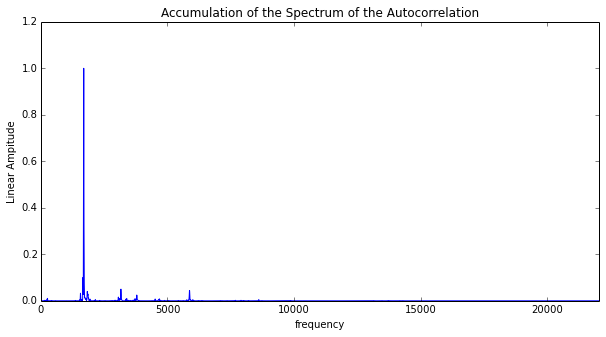
\includegraphics[width = 12cm]{BAK4_final_files/BAK4_final_12_1.png}
               \caption{The spectrum used for analysis}
               \label{pySpec}
           \end{center}
       \end{figure}
       
       
              
    % \begin{center}
    % \adjustimage{max size={0.9\linewidth}{0.9\paperheight}}{BAK4_final_files/BAK4_final_12_1.png}
    % \end{center}
    % { \hspace*{\fill} \\}
   
   \subsection{Pre-Processing}
\label{subsec:preprocess} 
    The spectral data needs to be smoothed for the proposed peak
finding algorithm to give meaningful results. The smoothing has to be
done with a linear phase FIR filter, so convolution with a symmetrical
kernel(a sinc function in this case) is performed. It is important that
this low-pass filter does preserve peak locations. In case of convolution with a
sinc function of length \(x\), the peaks will be delayed by \(x/2\). This delay
would mean that the detected frequencies would shift to the high end.
Thus, this is compensated below by use of the defined \textit{shift()}
function.

    \begin{Verbatim}[commandchars=\\\{\}]
{\color{incolor}In [{\color{incolor}29}]:} \PY{c}{\PYZsh{}A function for generating a Convolution Kernel}
         \PY{k}{def} \PY{n+nf}{sincKernel}\PY{p}{(}\PY{n}{length}\PY{p}{)}\PY{p}{:}
             \PY{n}{x} \PY{o}{=} \PY{n}{np}\PY{o}{.}\PY{n}{linspace}\PY{p}{(}\PY{o}{\PYZhy{}}\PY{l+m+mi}{1}\PY{p}{,}\PY{l+m+mi}{1}\PY{p}{,}\PY{n}{length}\PY{p}{)}
             \PY{n}{kernel} \PY{o}{=} \PY{p}{[}\PY{p}{]}
             \PY{k}{for} \PY{n}{i} \PY{o+ow}{in} \PY{n}{x}\PY{p}{:}
                 \PY{n}{kernel}\PY{o}{.}\PY{n}{append}\PY{p}{(}\PY{n}{np}\PY{o}{.}\PY{n}{sinc}\PY{p}{(}\PY{n}{i}\PY{p}{)}\PY{p}{)}
             \PY{k}{return} \PY{n}{kernel}
\end{Verbatim}

    \begin{Verbatim}[commandchars=\\\{\}]
{\color{incolor}In [{\color{incolor}30}]:} \PY{c}{\PYZsh{}Generating and plotting the Kernel}
         \PY{n}{convolutionLength} \PY{o}{=} \PY{l+m+mi}{20}
         \PY{n}{kernel} \PY{o}{=} \PY{n}{sincKernel}\PY{p}{(}\PY{n}{convolutionLength}\PY{p}{)}
         \PY{n}{n} \PY{o}{=} \PY{n+nb}{range}\PY{p}{(}\PY{n}{convolutionLength}\PY{p}{)}
         \PY{n}{plt}\PY{o}{.}\PY{n}{stem}\PY{p}{(}\PY{n}{n}\PY{p}{,} \PY{n}{kernel}\PY{p}{,} \PY{n}{linefmt}\PY{o}{=}\PY{l+s}{\PYZsq{}}\PY{l+s}{k}\PY{l+s}{\PYZsq{}}\PY{p}{,} \PY{n}{markerfmt}\PY{o}{=}\PY{l+s}{\PYZsq{}}\PY{l+s}{ko}\PY{l+s}{\PYZsq{}}\PY{p}{,} \PY{n}{basefmt}\PY{o}{=}\PY{l+s}{\PYZsq{}}\PY{l+s}{k\PYZhy{}\PYZhy{}}\PY{l+s}{\PYZsq{}}\PY{p}{)}
         \PY{n}{plt}\PY{o}{.}\PY{n}{grid}\PY{p}{(}\PY{n+nb+bp}{True}\PY{p}{)}
         \PY{n}{plt}\PY{o}{.}\PY{n}{axis}\PY{p}{(}\PY{p}{[}\PY{o}{\PYZhy{}}\PY{l+m+mi}{1}\PY{p}{,} \PY{n}{convolutionLength}\PY{p}{,}\PY{l+m+mi}{0}\PY{p}{,}\PY{l+m+mf}{1.1}\PY{p}{]}\PY{p}{)}
\end{Verbatim}


\begin{figure}[h]
    \begin{center}
        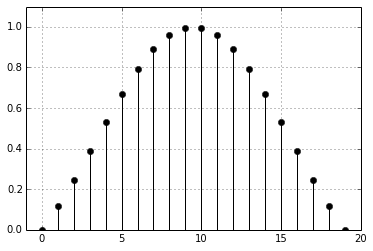
\includegraphics[width = 7cm]{BAK4_final_files/BAK4_final_15_0.png}
        \caption{The convolution kernel used to smooth the data}
        \label{kernel}
    \end{center}
\end{figure}



    % \begin{center}
    % \adjustimage{max size={0.9\linewidth}{0.9\paperheight}}{BAK4_final_files/BAK4_final_15_0.png}
    % \end{center}
    % { \hspace*{\fill} \\}

    After the convolution kernel has been created, the spectrum is filtered to obtain a smoothed version of it. After that, it is shifted to the left to compensate the delay introduced by the smoothing. Note that this is a filtering in the frequency domain, a lowpass filter running on the magnitude signal, it is not convolution in the time domain. One could also say here an amplitude modulation in the time domain happens. This AM approach does not provide the necessary control over the smoothing amount, which is why convolution in the frequency domain is performed.

    \begin{Verbatim}[commandchars=\\\{\}]
{\color{incolor}In [{\color{incolor}31}]:} \PY{n}{fig} \PY{o}{=} \PY{n}{plt}\PY{o}{.}\PY{n}{figure}\PY{p}{(}\PY{p}{)}
         \PY{n}{plt}\PY{o}{.}\PY{n}{axis}\PY{p}{(}\PY{p}{[}\PY{l+m+mi}{0}\PY{p}{,} \PY{l+m+mi}{6000}\PY{p}{,} \PY{l+m+mi}{0}\PY{p}{,} \PY{l+m+mf}{0.2}\PY{p}{]}\PY{p}{)}
         \PY{n}{ax} \PY{o}{=} \PY{n}{fig}\PY{o}{.}\PY{n}{add\PYZus{}subplot}\PY{p}{(}\PY{l+m+mi}{111}\PY{p}{)}
         \PY{c}{\PYZsh{}\PYZhy{}\PYZhy{}\PYZhy{}\PYZhy{}\PYZhy{}\PYZhy{}\PYZhy{}IndexSIgnal}
         \PY{n}{x2} \PY{o}{=} \PY{n}{np}\PY{o}{.}\PY{n}{linspace}\PY{p}{(}\PY{l+m+mi}{0}\PY{p}{,} \PY{n}{sr}\PY{o}{/}\PY{l+m+mi}{2}\PY{p}{,} \PY{n}{frameSize}\PY{p}{)}
         \PY{c}{\PYZsh{}\PYZhy{}\PYZhy{}plot OriginalFrame}
         \PY{n}{plt}\PY{o}{.}\PY{n}{plot}\PY{p}{(}\PY{n}{x2}\PY{p}{,} \PY{n}{frame}\PY{p}{,} \PY{n}{color}\PY{o}{=}\PY{l+s}{\PYZsq{}}\PY{l+s}{0.1}\PY{l+s}{\PYZsq{}}\PY{p}{,} \PY{n}{label}\PY{o}{=} \PY{l+s}{\PYZdq{}}\PY{l+s}{original}\PY{l+s}{\PYZdq{}}\PY{p}{,} \PY{n}{linewidth}\PY{o}{=}\PY{l+m+mf}{0.5}\PY{p}{)}
         \PY{c}{\PYZsh{} \PYZhy{}\PYZhy{}\PYZhy{}\PYZhy{}\PYZhy{}Convolution}
         \PY{n}{conv} \PY{o}{=} \PY{n}{np}\PY{o}{.}\PY{n}{convolve}\PY{p}{(}\PY{n}{frame}\PY{p}{,}\PY{n}{kernel}\PY{p}{)}
         \PY{c}{\PYZsh{}truncating result, a convolved }
         \PY{c}{\PYZsh{}signal always has length input length+kernel length:}
         \PY{n}{conv} \PY{o}{=} \PY{n}{conv}\PY{p}{[}\PY{p}{:}\PY{l+m+mi}{4096}\PY{p}{]}
         \PY{c}{\PYZsh{} \PYZhy{}\PYZhy{}\PYZhy{}\PYZhy{}\PYZhy{}\PYZhy{}post\PYZhy{}attenuate}
         \PY{n}{conv}\PY{p}{[}\PY{p}{:}\PY{p}{]} \PY{o}{=} \PY{p}{[}\PY{n}{x}\PY{o}{*}\PY{l+m+mf}{0.25} \PY{k}{for} \PY{n}{x} \PY{o+ow}{in} \PY{n}{conv}\PY{p}{]}
         
         \PY{c}{\PYZsh{} a negative delay applied to the result}
         \PY{c}{\PYZsh{} of the convolution as a compensation.}
         \PY{k}{def} \PY{n+nf}{shift}\PY{p}{(}\PY{n}{array}\PY{p}{,} \PY{n}{n}\PY{p}{)}\PY{p}{:}
             \PY{k}{for} \PY{n}{i} \PY{o+ow}{in} \PY{n+nb}{range}\PY{p}{(}\PY{n+nb}{len}\PY{p}{(}\PY{n}{array}\PY{p}{)}\PY{p}{)}\PY{p}{:}
                 \PY{n}{index} \PY{o}{=} \PY{p}{(}\PY{n}{i}\PY{o}{+}\PY{n}{n}\PY{p}{)}
                 \PY{k}{if} \PY{n}{index} \PY{o}{\PYZlt{}} \PY{l+m+mi}{0}\PY{p}{:}
                     \PY{n}{array}\PY{p}{[}\PY{n}{i}\PY{p}{]} \PY{o}{=} \PY{l+m+mi}{0}
                 \PY{k}{elif} \PY{n}{index} \PY{o}{\PYZgt{}}\PY{o}{=} \PY{n+nb}{len}\PY{p}{(}\PY{n}{array}\PY{p}{)}\PY{p}{:}
                     \PY{n}{array}\PY{p}{[}\PY{n}{i}\PY{p}{]} \PY{o}{=} \PY{l+m+mi}{0}
                 \PY{k}{else}\PY{p}{:}
                     \PY{n}{array}\PY{p}{[}\PY{n}{i}\PY{p}{]}\PY{o}{=} \PY{n}{array}\PY{p}{[}\PY{n}{i}\PY{o}{+}\PY{n}{n}\PY{p}{]}
             \PY{k}{return} \PY{n}{array}
         \PY{c}{\PYZsh{}applying the compensation delay:}
         \PY{n}{filtered} \PY{o}{=} \PY{n}{shift}\PY{p}{(}\PY{n}{conv}\PY{p}{,}\PY{n}{convolutionLength}\PY{o}{/}\PY{l+m+mi}{2}\PY{p}{)}
         \PY{c}{\PYZsh{}\PYZhy{}\PYZhy{}plotting}
         \PY{n}{plt}\PY{o}{.}\PY{n}{plot}\PY{p}{(}\PY{n}{x2}\PY{p}{,} \PY{n}{filtered}\PY{p}{,} \PY{l+s}{\PYZsq{}}\PY{l+s}{k}\PY{l+s}{\PYZsq{}}\PY{p}{,} \PY{n}{label}\PY{o}{=} \PY{l+s}{\PYZdq{}}\PY{l+s}{filtered}\PY{l+s}{\PYZdq{}}\PY{p}{,} \PY{n}{linewidth}\PY{o}{=}\PY{l+m+mf}{2.}\PY{p}{)}
         \PY{n}{plt}\PY{o}{.}\PY{n}{title}\PY{p}{(}\PY{l+s}{\PYZsq{}}\PY{l+s}{Convolution of the Spectrum}\PY{l+s}{\PYZsq{}}\PY{p}{)}\PY{p}{;}
         \PY{n}{ax}\PY{o}{.}\PY{n}{set\PYZus{}xlabel}\PY{p}{(}\PY{l+s}{\PYZsq{}}\PY{l+s}{frequency}\PY{l+s}{\PYZsq{}}\PY{p}{)}
         \PY{n}{ax}\PY{o}{.}\PY{n}{set\PYZus{}ylabel}\PY{p}{(}\PY{l+s}{\PYZsq{}}\PY{l+s}{Linear Ampitude}\PY{l+s}{\PYZsq{}}\PY{p}{)}
         \PY{n}{plt}\PY{o}{.}\PY{n}{legend}\PY{p}{(}\PY{n}{bbox\PYZus{}to\PYZus{}anchor}\PY{o}{=}\PY{p}{(}\PY{l+m+mi}{1}\PY{p}{,} \PY{l+m+mi}{1}\PY{p}{)}\PY{p}{,} \PY{n}{loc}\PY{o}{=}\PY{l+m+mi}{1}\PY{p}{,} \PY{n}{borderaxespad}\PY{o}{=}\PY{l+m+mf}{0.}\PY{p}{)}
\end{Verbatim}


\begin{figure}[h]
    \begin{center}
        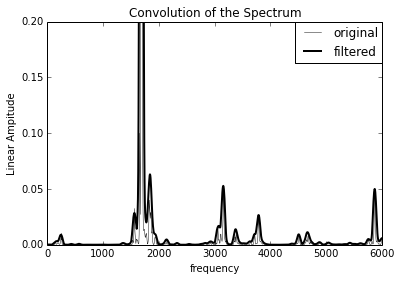
\includegraphics[width = 12cm]{BAK4_final_files/BAK4_final_16_0.png}
        \caption{The smoothed spectrum}
        \label{smoothSpectrum}
    \end{center}
\end{figure}



    % \begin{center}
    % \adjustimage{max size={0.9\linewidth}{0.9\paperheight}}{BAK4_final_files/BAK4_final_16_0.png}
    % \end{center}
    % { \hspace*{\fill} \\}
    
    \subsection{Actual Peak Finding}
\label{subsec:peakfinding}
    Below, the actual peak finding function is defined. This algorithm just looks for the maximum value in the spectrum, saves its index and deletes it from the array. After that it \glqq{}goes\grqq{} to the right, deleting everything until the derivative goes above a certain threshold(until it meets a more or less constant spot or a starting peak). Then it \glqq{}goes\grqq{} to the left, deleting everything until the derivative goes below a certain threshold. Deleting here means just to set the values to zero and therefore eliminating the indices for future maximum lookups. After that it looks for the maximum value in the resulting curve again and starts deleting again. Therefore, as long as the function is smoothed and the two parameters are set correctly, the algorithm will reliably find local maxima.

    \begin{Verbatim}[commandchars=\\\{\}]
{\color{incolor}In [{\color{incolor}32}]:} \PY{c}{\PYZsh{}a function for obtaining the derivative of an array}
         \PY{k}{def} \PY{n+nf}{delta}\PY{p}{(}\PY{n}{data}\PY{p}{)}\PY{p}{:}
             \PY{n}{delta} \PY{o}{=} \PY{p}{[}\PY{p}{]}
             \PY{k}{for} \PY{n}{i} \PY{o+ow}{in} \PY{n+nb}{range}\PY{p}{(}\PY{n+nb}{len}\PY{p}{(}\PY{n}{data}\PY{p}{)}\PY{p}{)}\PY{p}{:}
                 \PY{k}{if} \PY{n}{i} \PY{o}{!=} \PY{l+m+mi}{0}\PY{p}{:}
                     \PY{n}{d} \PY{o}{=} \PY{n}{data}\PY{p}{[}\PY{n}{i}\PY{p}{]} \PY{o}{\PYZhy{}} \PY{n}{data}\PY{p}{[}\PY{n}{i} \PY{o}{\PYZhy{}} \PY{l+m+mi}{1}\PY{p}{]} 
                 \PY{k}{else}\PY{p}{:} 
                     \PY{n}{d} \PY{o}{=} \PY{l+m+mi}{0}
                 \PY{n}{delta}\PY{o}{.}\PY{n}{append}\PY{p}{(}\PY{n}{d}\PY{p}{)}
             \PY{k}{return} \PY{n}{delta}
         
         \PY{k}{def} \PY{n+nf}{findPeaks}\PY{p}{(}\PY{n}{data}\PY{p}{,} \PY{n}{iterarions}\PY{p}{,}\PY{n}{thresh}\PY{p}{)}\PY{p}{:}
         	\PY{k+kn}{import} \PY{n+nn}{numpy} \PY{k+kn}{as} \PY{n+nn}{np}
         	\PY{k+kn}{import} \PY{n+nn}{copy}
         	\PY{n}{tdata} \PY{o}{=} \PY{n}{copy}\PY{o}{.}\PY{n}{copy}\PY{p}{(}\PY{n}{data}\PY{p}{)}
         	\PY{n}{length} \PY{o}{=} \PY{n+nb}{len}\PY{p}{(}\PY{n}{data}\PY{p}{)}
         	\PY{n}{peaks} \PY{o}{=} \PY{p}{[}\PY{p}{]}
         	\PY{n}{delt} \PY{o}{=} \PY{n}{delta}\PY{p}{(}\PY{n}{data}\PY{p}{)}
         
         	\PY{k}{for} \PY{n}{i} \PY{o+ow}{in} \PY{n+nb}{range}\PY{p}{(}\PY{n}{iterarions}\PY{p}{)}\PY{p}{:}
         		
         		\PY{n}{tmax} \PY{o}{=} \PY{n}{np}\PY{o}{.}\PY{n}{argmax}\PY{p}{(}\PY{n}{tdata}\PY{p}{)}
         		\PY{n}{peaks}\PY{o}{.}\PY{n}{append}\PY{p}{(}\PY{n}{tmax}\PY{p}{)}
         		\PY{n}{deriv} \PY{o}{=} \PY{o}{\PYZhy{}}\PY{l+m+mf}{1.}
         		\PY{c}{\PYZsh{}thresh = 0.001}
         		\PY{n}{j} \PY{o}{=} \PY{l+m+mi}{1}
         		\PY{n}{tdata}\PY{p}{[}\PY{n}{tmax}\PY{p}{]}\PY{o}{=} \PY{l+m+mi}{0}
         		\PY{k}{while} \PY{p}{(}\PY{n}{deriv}\PY{p}{)}\PY{o}{\PYZlt{}}\PY{n}{thresh} \PY{o+ow}{and} \PY{n}{j} \PY{o}{\PYZlt{}} \PY{l+m+mi}{100}\PY{p}{:}
         			\PY{n}{index} \PY{o}{=} \PY{n}{np}\PY{o}{.}\PY{n}{clip}\PY{p}{(}\PY{n}{tmax}\PY{o}{+}\PY{n}{j}\PY{p}{,} \PY{l+m+mi}{0}\PY{p}{,} \PY{n}{length}\PY{o}{\PYZhy{}}\PY{l+m+mi}{1}\PY{p}{)}
         			\PY{n}{deriv} \PY{o}{=} \PY{n}{delt}\PY{p}{[}\PY{n}{index}\PY{o}{+}\PY{l+m+mi}{1}\PY{p}{]}
         			\PY{n}{tdata}\PY{p}{[}\PY{n}{index}\PY{p}{]} \PY{o}{=} \PY{l+m+mi}{0}
         			\PY{n}{j} \PY{o}{=} \PY{n}{j} \PY{o}{+} \PY{l+m+mi}{1} 
         		
         		\PY{n}{j} \PY{o}{=} \PY{l+m+mi}{1}
         		\PY{n}{deriv} \PY{o}{=} \PY{l+m+mf}{1.}
         		\PY{k}{while} \PY{n}{deriv}\PY{o}{\PYZgt{}}\PY{p}{(}\PY{n}{thresh}\PY{o}{*}\PY{o}{\PYZhy{}}\PY{l+m+mi}{1}\PY{p}{)} \PY{o+ow}{and} \PY{n}{j} \PY{o}{\PYZlt{}} \PY{l+m+mi}{100}\PY{p}{:}
         			\PY{n}{index} \PY{o}{=} \PY{n}{np}\PY{o}{.}\PY{n}{clip}\PY{p}{(}\PY{n}{tmax}\PY{o}{\PYZhy{}}\PY{n}{j}\PY{p}{,} \PY{l+m+mi}{0}\PY{p}{,} \PY{n}{length}\PY{p}{)}
         			\PY{n}{deriv} \PY{o}{=} \PY{n}{delt}\PY{p}{[}\PY{n}{index}\PY{p}{]}
         			\PY{n}{tdata}\PY{p}{[}\PY{n}{index}\PY{p}{]} \PY{o}{=} \PY{l+m+mi}{0}
         			\PY{n}{j} \PY{o}{=} \PY{n}{j} \PY{o}{+} \PY{l+m+mi}{1}
         	\PY{k}{return} \PY{n}{peaks}\PY{p}{,} \PY{n}{tdata}
         
         \PY{c}{\PYZsh{}A helper function, just for plotting}
         \PY{k}{def} \PY{n+nf}{markers}\PY{p}{(}\PY{n}{data}\PY{p}{,} \PY{n}{peaks}\PY{p}{,} \PY{n}{length}\PY{p}{)}\PY{p}{:}
         	\PY{k+kn}{import} \PY{n+nn}{numpy} \PY{k+kn}{as} \PY{n+nn}{np}
         	\PY{n}{markers}\PY{o}{=} \PY{n}{np}\PY{o}{.}\PY{n}{zeros}\PY{p}{(}\PY{n}{length}\PY{p}{)}
         	\PY{n}{markers} \PY{o}{=} \PY{n}{markers}\PY{o}{\PYZhy{}}\PY{l+m+mi}{1}
         	\PY{k}{for} \PY{n}{i} \PY{o+ow}{in} \PY{n+nb}{range}\PY{p}{(}\PY{n+nb}{len}\PY{p}{(}\PY{n}{peaks}\PY{p}{)}\PY{p}{)}\PY{p}{:}
         		\PY{n}{markers}\PY{p}{[}\PY{n}{peaks}\PY{p}{[}\PY{n}{i}\PY{p}{]}\PY{p}{]}\PY{o}{=}\PY{n}{data}\PY{p}{[}\PY{n}{peaks}\PY{p}{[}\PY{n}{i}\PY{p}{]}\PY{p}{]}
         	\PY{k}{return} \PY{n}{markers}		
\end{Verbatim}

    The parameters of the peak detection are set: The number of
desired/estimated peaks and a threshold value, that regulates the
algorithm's sensitivity to the values of the derivative of the input:

    \begin{Verbatim}[commandchars=\\\{\}]
{\color{incolor}In [{\color{incolor}33}]:} \PY{n}{numberOfPeaks} \PY{o}{=} \PY{l+m+mi}{15}
         \PY{n}{threshold} \PY{o}{=} \PY{l+m+mf}{0.001}
\end{Verbatim}

    Finally, the peaks are dected:

    \begin{Verbatim}[commandchars=\\\{\}]
{\color{incolor}In [{\color{incolor}34}]:} \PY{n}{result} \PY{o}{=} \PY{n}{findPeaks}\PY{p}{(}\PY{n}{filtered}\PY{p}{,}\PY{n}{numberOfPeaks}\PY{p}{,}\PY{n}{threshold}\PY{p}{)}
         \PY{n}{peaks} \PY{o}{=} \PY{n}{result}\PY{p}{[}\PY{l+m+mi}{0}\PY{p}{]}
         \PY{n}{tdata} \PY{o}{=} \PY{n}{result}\PY{p}{[}\PY{l+m+mi}{1}\PY{p}{]}
         \PY{n}{marks} \PY{o}{=} \PY{n}{markers}\PY{p}{(}\PY{n}{filtered}\PY{p}{,} \PY{n}{peaks}\PY{p}{,} \PY{n}{frameSize}\PY{p}{)}
         \PY{n}{peakFreqs} \PY{o}{=} \PY{n}{binToFreq}\PY{p}{(}\PY{n}{peaks}\PY{p}{,} \PY{n}{sr}\PY{p}{,}\PY{n}{frameSize}\PY{p}{)}
         \PY{n}{peakFreqs}\PY{o}{=}\PY{n}{np}\PY{o}{.}\PY{n}{sort}\PY{p}{(}\PY{n}{peakFreqs}\PY{p}{)}
         \PY{k}{print} \PY{l+s}{\PYZdq{}}\PY{l+s}{Detected Peak Frequencies:}\PY{l+s}{\PYZdq{}}\PY{o}{+}\PY{l+s}{\PYZdq{}}\PY{l+s+se}{\PYZbs{}n}\PY{l+s}{\PYZdq{}}\PY{o}{+}\PY{n+nb}{str}\PY{p}{(}\PY{n}{peakFreqs}\PY{p}{)}
\end{Verbatim}

    \begin{Verbatim}[commandchars=\\\{\}]
Detected Peak Frequencies:
[   247.63183594   1561.15722656   1684.97314453   1841.08886719
   3154.61425781   3375.32958984   3784.46044922   4505.82275391
   4661.93847656   5867.79785156   7671.20361328   8602.51464844
   9846.05712891  13135.25390625  13727.41699219]
    \end{Verbatim}

    And plotted:

    \begin{Verbatim}[commandchars=\\\{\}]
{\color{incolor}In [{\color{incolor}36}]:} \PY{n}{fig} \PY{o}{=} \PY{n}{plt}\PY{o}{.}\PY{n}{figure}\PY{p}{(}\PY{p}{)}
         \PY{n}{ax} \PY{o}{=} \PY{n}{fig}\PY{o}{.}\PY{n}{add\PYZus{}subplot}\PY{p}{(}\PY{l+m+mi}{111}\PY{p}{)}
         \PY{n}{plt}\PY{o}{.}\PY{n}{axis}\PY{p}{(}\PY{p}{[}\PY{l+m+mi}{0}\PY{p}{,} \PY{l+m+mi}{6000}\PY{p}{,} \PY{l+m+mi}{0}\PY{p}{,} \PY{l+m+mf}{0.2}\PY{p}{]}\PY{p}{)}
         \PY{n}{plt}\PY{o}{.}\PY{n}{plot}\PY{p}{(}\PY{n}{x2}\PY{p}{,} \PY{n}{marks}\PY{p}{,} \PY{l+s}{\PYZdq{}}\PY{l+s}{rx}\PY{l+s}{\PYZdq{}}\PY{p}{,}\PY{n}{markersize}\PY{o}{=}\PY{l+m+mi}{15}\PY{p}{,} \PY{n}{label}\PY{o}{=}\PY{l+s}{\PYZdq{}}\PY{l+s}{detected Peaks}\PY{l+s}{\PYZdq{}}\PY{p}{)}
         \PY{n}{plt}\PY{o}{.}\PY{n}{plot}\PY{p}{(}\PY{n}{x2}\PY{p}{,} \PY{n}{filtered}\PY{p}{,} \PY{l+s}{\PYZdq{}}\PY{l+s}{k\PYZhy{}.}\PY{l+s}{\PYZdq{}}\PY{p}{,} \PY{n}{label}\PY{o}{=}\PY{l+s}{\PYZdq{}}\PY{l+s}{Smoothed Spectrum}\PY{l+s}{\PYZdq{}}\PY{p}{)}
         \PY{n}{plt}\PY{o}{.}\PY{n}{plot}\PY{p}{(}\PY{n}{x2}\PY{p}{,} \PY{n}{frame}\PY{p}{,} \PY{l+s}{\PYZdq{}}\PY{l+s}{k}\PY{l+s}{\PYZdq{}}\PY{p}{,} \PY{n}{label}\PY{o}{=}\PY{l+s}{\PYZdq{}}\PY{l+s}{Original Spectrum}\PY{l+s}{\PYZdq{}}\PY{p}{)}
         \PY{n}{ax}\PY{o}{.}\PY{n}{set\PYZus{}xlabel}\PY{p}{(}\PY{l+s}{\PYZsq{}}\PY{l+s}{frequency}\PY{l+s}{\PYZsq{}}\PY{p}{)}
         \PY{n}{ax}\PY{o}{.}\PY{n}{set\PYZus{}ylabel}\PY{p}{(}\PY{l+s}{\PYZsq{}}\PY{l+s}{Linear Ampitude}\PY{l+s}{\PYZsq{}}\PY{p}{)}
         \PY{n}{plt}\PY{o}{.}\PY{n}{legend}\PY{p}{(}\PY{n}{bbox\PYZus{}to\PYZus{}anchor}\PY{o}{=}\PY{p}{(}\PY{l+m+mi}{1}\PY{p}{,} \PY{l+m+mi}{1}\PY{p}{)}\PY{p}{,} \PY{n}{loc}\PY{o}{=}\PY{l+m+mi}{1}\PY{p}{,} \PY{n}{borderaxespad}\PY{o}{=}\PY{l+m+mf}{0.}\PY{p}{)}
\end{Verbatim}

%             \begin{Verbatim}[commandchars=\\\{\}]
% {\color{outcolor}Out[{\color{outcolor}36}]:} <matplotlib.legend.Legend at 0x111482590>
% \end{Verbatim}

        \begin{figure}[h]
            \begin{center}
                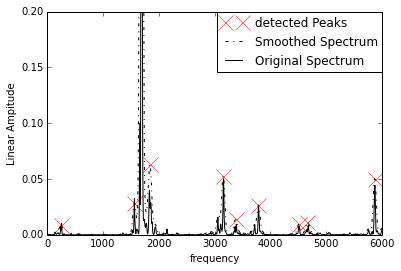
\includegraphics[width = 14cm]{BAK4_final_files/BAK4_final_23_1.png}
                \caption{detected peaks}
                \label{detected}
            \end{center}
        \end{figure}
        
        
                
    % \begin{center}
    % \adjustimage{max size={0.9\linewidth}{0.9\paperheight}}{BAK4_final_files/BAK4_final_23_1.png}
    % \end{center}
    % { \hspace*{\fill} \\}
    
%     \begin{Verbatim}[commandchars=\\\{\}]
% {\color{incolor}In [{\color{incolor}35}]:} 
% \end{Verbatim}

%     \begin{Verbatim}[commandchars=\\\{\}]
% {\color{incolor}In [{\color{incolor}35}]:} 
% \end{Verbatim}

%     \begin{Verbatim}[commandchars=\\\{\}]
% {\color{incolor}In [{\color{incolor}35}]:} 
% \end{Verbatim}

%     \begin{Verbatim}[commandchars=\\\{\}]
% {\color{incolor}In [{\color{incolor}}]:} 
% \end{Verbatim}


    % Add a bibliography block to the postdoc
    
    
    
    % \end{document}
